\documentclass[a4paper, 11pt, parskip=half]{scrreprt}

\usepackage[automark]{scrlayer-scrpage}         % Headings
\usepackage{DejaVuSerif}                        % Default font
\usepackage{DejaVuSans}                         % Headers font
\usepackage{sourcecodepro}                      % Monospace font
\usepackage[utf8]{inputenc}                     % Input encoding
\usepackage[T1]{fontenc}                        % Output encoding
\usepackage{graphicx}                           % Pictures
\usepackage{listings}                           % Code snippets
\usepackage{hyperref}                           % Make strings clickable
\usepackage{amsmath,amsfonts,stmaryrd,amssymb}  % Math packages
\usepackage{amsthm}                             % Definitions, theorems, corollaries, ...
\usepackage{mathtools}                          % Math stuff
\usepackage[usenames,dvipsnames,table]{xcolor}  % Colors
\usepackage[toc,page]{appendix}                 % Support for appendices
\usepackage[chapter]{algorithm}                 % Pseudocode headers
\usepackage{algpseudocode}                      % Pseudocode
\usepackage{pdfpages}                           % Embed external pdf
\usepackage{wrapfig}                            % Wrap text around figures
\usepackage{multicol}                           % Used for multicolumn itemize
\usepackage{multirow}                           % Used for multirow in tables
\usepackage{longtable}                          % Tables can spread over multiple pages
\usepackage{enumerate}                          % Custom item numbers for enumerations
\usepackage[framemethod=tikz]{mdframed}         % Allows defining custom boxed/framed environments
\usepackage{tocloft}                            % TOC spacing


% TODO: REMOVE
\usepackage{lipsum}
\usepackage{blindtext}



%----------------------------------------------------------------------------------------
%	DOCUMENT SETTINGS
%----------------------------------------------------------------------------------------

\areaset{17cm}{22.5cm}              % Set page width and height
\graphicspath{{./figures/}}         % Set path for figures
\setlength{\cftchapnumwidth}{2em}   % Set chapter numwidth
\setlength{\cftsecnumwidth}{3em}    % Set section numwidth
\setlength{\cftsubsecnumwidth}{4em} % Set subsection numwidth
\hypersetup{linktoc=all}            % Set TOC clickable

\lstset{ 
    belowcaptionskip=\baselineskip,
    aboveskip=\baselineskip,
    breaklines=true,
    frame=l,
    xleftmargin=0.5in,
    showstringspaces=false,
    basicstyle=\footnotesize\ttfamily,
    keywordstyle=\bfseries\color{green!40!black},
    commentstyle=\color{MidnightBlue},
    stringstyle=\color{BrickRed},
    numberstyle=\color{Cyan!50!Black},
    numbers=left,
    tabsize=4
}

\theoremstyle{definition}
\newtheorem{definition}{Definition}[chapter]
\newtheorem{theorem}{Theorem}[chapter]
\newtheorem{corollary}{Corollary}[theorem]


%----------------------------------------------------------------------------------------
%	COMMAND LINE ENVIRONMENT
%----------------------------------------------------------------------------------------

% Usage:
% \begin{commandline}
%	\begin{verbatim}
%		$ ls
%		
%		Applications	Desktop	...
%	\end{verbatim}
% \end{commandline}

\mdfdefinestyle{commandline}{
	leftmargin=10pt,
	rightmargin=10pt,
	innerleftmargin=15pt,
	middlelinecolor=black!50!white,
	middlelinewidth=2pt,
	frametitlerule=false,
	backgroundcolor=black!5!white,
	frametitle={Command line},
	frametitlefont={\normalfont\ttfamily\color{white}\hspace{-1em}},
	frametitlebackgroundcolor=black!50!white,
	nobreak,
}

% Define a custom environment for command-line snapshots
\newenvironment{commandline}{
	\medskip
	\begin{mdframed}[style=commandline]
	\footnotesize
}{
	\end{mdframed}
	\medskip
}


%----------------------------------------------------------------------------------------
%	FILE CONTENTS ENVIRONMENT
%----------------------------------------------------------------------------------------

% Usage:
% \begin{file}[optional filename, defaults to "File"]
%	File contents, for example, with a listings environment
% \end{file}

\mdfdefinestyle{file}{
	innertopmargin=1.6\baselineskip,
	innerbottommargin=0.28\baselineskip,
	topline=false, bottomline=false,
	leftline=false, rightline=false,
	leftmargin=2cm,
	rightmargin=2cm,
	singleextra={%
		\draw[fill=black!10!white](P)++(0,-1.3em)rectangle(P-|O);
		\node[anchor=north west]
		at(P-|O){\footnotesize\ttfamily\mdfilename};
		%
		\def\l{1.5em}
		\draw(O-|P)++(-\l,0)--++(\l,\l)--(P)--(P-|O)--(O)--cycle;
		\draw(O-|P)++(-\l,0)--++(0,\l)--++(\l,0);
	},
	nobreak,
}

% Define a custom environment for file contents
\newenvironment{file}[1][File]{ % Set the default filename to "File"
	\medskip
	\newcommand{\mdfilename}{#1}
	\begin{mdframed}[style=file]
}{
	\end{mdframed}
	\medskip
}


%----------------------------------------------------------------------------------------
%	NUMBERED QUESTIONS ENVIRONMENT
%----------------------------------------------------------------------------------------

% Usage:
% \begin{question}[optional title]
%	Question contents
% \end{question}

\mdfdefinestyle{question}{
	innertopmargin=1.2\baselineskip,
	innerbottommargin=0.8\baselineskip,
	roundcorner=5pt,
	nobreak,
	singleextra={%
		\draw(P-|O)node[xshift=1em,anchor=west,fill=white,draw,rounded corners=5pt]{%
		Question \theQuestion\questionTitle};
	},
}

\newcounter{Question} % Stores the current question number that gets iterated with each new question

% Define a custom environment for numbered questions
\newenvironment{question}[1][\unskip]{
	\bigskip
	\stepcounter{Question}
	\newcommand{\questionTitle}{~#1}
	\begin{mdframed}[style=question]
}{
	\end{mdframed}
	\medskip
}


%----------------------------------------------------------------------------------------
%	BOXED PARAGRAPH ENVIRONMENT
%----------------------------------------------------------------------------------------

% Usage:
% \begin{boxedpar}[optional title]
%	Question contents
% \end{boxedpar}

\mdfdefinestyle{boxedpar}{
	innertopmargin=1.2\baselineskip,
	innerbottommargin=0.8\baselineskip,
	roundcorner=5pt,
	nobreak,
	singleextra={%
		\draw(P-|O)node[xshift=1em,anchor=west,fill=white,draw,rounded corners=5pt]{%
		\textit{\boxTitle}};
	},
}

% Define a custom environment for numbered questions
\newenvironment{boxedpar}[1][in-depth]{
	\bigskip
	\newcommand{\boxTitle}{#1}
	\begin{mdframed}[style=boxedpar]
}{
	\end{mdframed}
	\medskip
}


%----------------------------------------------------------------------------------------
%	ROUNDED BOX ENVIRONMENT
%----------------------------------------------------------------------------------------

% Usage:
% \begin{roundedbox}
%	Contents
% \end{roundedbox}

\mdfdefinestyle{roundedbox}{
	innertopmargin=0.5\baselineskip,
	innerbottommargin=0.5\baselineskip,
	roundcorner=5pt,
	nobreak,
}

% Define a custom environment for numbered questions
\newenvironment{roundedbox}{
	\bigskip
	\begin{mdframed}[style=roundedbox]
}{
	\end{mdframed}
	\medskip
}


%----------------------------------------------------------------------------------------
%	WARNING TEXT ENVIRONMENT
%----------------------------------------------------------------------------------------

% Usage:
% \begin{warn}[optional title, defaults to "Warning:"]
%	Contents
% \end{warn}

\mdfdefinestyle{warning}{
	topline=false, bottomline=false,
	leftline=false, rightline=false,
	nobreak,
	singleextra={%
		\draw(P-|O)++(-0.5em,0)node(tmp1){};
		\draw(P-|O)++(0.5em,0)node(tmp2){};
		\fill[black,rotate around={45:(P-|O)}](tmp1)rectangle(tmp2);
		\node at(P-|O){\color{white}\scriptsize\textbf !};
		\draw[very thick](P-|O)++(0,-1em)--(O);%--(O-|P);
	}
}

% Define a custom environment for warning text
\newenvironment{warn}[1][Warning:]{ % Set the default warning to "Warning:"
	\medskip
	\begin{mdframed}[style=warning]
		\noindent{\textbf{#1}}
}{
	\end{mdframed}
}


%----------------------------------------------------------------------------------------
%	INFORMATION ENVIRONMENT
%----------------------------------------------------------------------------------------

% Usage:
% \begin{info}[optional title, defaults to "Info:"]
% 	contents
% 	\end{info}

\mdfdefinestyle{info}{%
	topline=false, bottomline=false,
	leftline=false, rightline=false,
	nobreak,
	singleextra={%
		\fill[black](P-|O)circle[radius=0.4em];
		\node at(P-|O){\color{white}\scriptsize\textbf i};
		\draw[very thick](P-|O)++(0,-0.8em)--(O);%--(O-|P);
	}
}

% Define a custom environment for information
\newenvironment{info}[1][Info:]{ % Set the default title to "Info:"
	\medskip
	\begin{mdframed}[style=info]
		\noindent{\textbf{#1}}
}{
	\end{mdframed}
}


%----------------------------------------------------------------------------------------
%	LINEDQUOTE ENVIRONMENT
%----------------------------------------------------------------------------------------

% Usage:
% \begin{linedquote}
% 	contents
% 	\end{linedquote}

\mdfdefinestyle{linedquote}{%
	topline=false, bottomline=false,
	leftline=false, rightline=false,
	nobreak,
	singleextra={%
		\draw[very thick](P-|O)++(0,0)--(O);%--(O-|P);
	}
}

% Define a custom environment
\newenvironment{linedquote}{
	\begin{mdframed}[style=linedquote]
}{
	\end{mdframed}
}


%----------------------------------------------------------------------------------------
%	TITLE PAGE
%----------------------------------------------------------------------------------------

\publishers{
    \begin{figure}[t]
        \centering
        
\includegraphics[width=0.9\linewidth, keepaspectratio]{logo}
    \end{figure}
}
\title{Smart Tourist}
\subtitle{Design and Implementation of Mobile Applications\\Design Document}
\date{A.Y. 2019/2020}
\author{Fabio Codiglioni, Alessandro Nichelini}



%----------------------------------------------------------------------------------------
%	DOCUMENT
%----------------------------------------------------------------------------------------

\begin{document}

% Title page and TOC
\pagenumbering{gobble}
\maketitle
%\shipout\null           % Blank page
\pagenumbering{roman}
\tableofcontents
\newpage
\pagenumbering{arabic}


% Body

\chapter{Introduction}
This is the \textit{design document} (DD) of the \textbf{\textit{Smart Tourist}} iOS application developed by \textit{Fabio Codiglioni} and \textit{Alessandro Nichelini} in the context of the \textit{Design and Implementation of Mobile Application} course at Politecnico di Milano. The authors have been tutored by Bending Spoons for the usage of some technologies that are described later.\\
The document explains the most important design choices we made and the motivations behind them, with specific focus on the Redux-like architecture adopted.




\chapter{General Overview}
Smart Tourist is a multi-device application for iOS and iPadOS.

\section{Assignment}
For the reader convenience, the assignment is reported below:
\begin{warn}[Assignement:]
	 Smart Tourist
	 \\\\Help your users when they are exploring new cities!
	 \\\\By using the localisation systems on the smartphones and the google places API, notify the user when something interesting is nearby.
	 \\\\Connect to wikipedia, to retrieve interesting informations on the point of interest selected.
	 \\\\Search and filters among several interesting places of the city you are visiting, save them as favourites so you can check on them later.
	 \\\\Attach some pictures to those pins and eventually share them with your friends!
\end{warn}

 \section{Features description}
 \subsection{Exploring}
 The user is given with a navigation map filled with the city's point of interest. She has the chance to control which attraction to see on a map. She can choose between \textit{Nearest places}, \textit{Popular places} and \textit{Favourites}. Each attraction is shown on the map and in a table view. They are clickable from both position to open  the corresponding detail view.
 \\\\In the map, two circles are displayed to help the user better understand distances. These circles correspond to the distance she can cover in 5 and 15 minutes. Circles' radius is automatically updated with information from user profile and thus they fit always with user's pace.
 
 \subsection{Dynamical exploring}
 SmartTourist works well in both crowded cities and small towns. The user will be always provided with a right amount of attractions. Where not so many attractions are available, the app will automatically show her less known attraction and particular point of interest.
 
 \subsection{Learning}
 The user can open the detail view of both the city and attractions. She will be provided with useful information about the point of interest such as pictures, Wikipedia description, useful links and a shortcut to open turn-by-turn navigation.
 
 \subsection{Notifications}
 The user is notified when she is nearby a "top location". The notification comes with a picture of the attraction and lets her either to open the the detail view of the attraction or to open turn-by-turn navigation. 
 
 \subsection{Keep track of favourite attractions}
 The user can view the attraction of her current city or she can have a preview of other cities attractions. In both case she can keep track of them by adding them in the list of favourite attractions. The user is also provided the ability to open a worldwide map with all her favourite places.

\subsection{Contribute (proof of concept)}
SmartTourist is manly based on free data. When a detailed description is missing, the user is given the chance to contribute.


\chapter{Architectural design}




\chapter{Data design}




\chapter{User interface}
\section{Screenshot}
Here follow some screenshot of the application in both Light and Dark mode.

\subsection{Mapview}
\subsubsection{Mapview - nearest}
\begin{figure}[H]
	\centering
	\begin{minipage}{.5\textwidth}
  	\centering
  	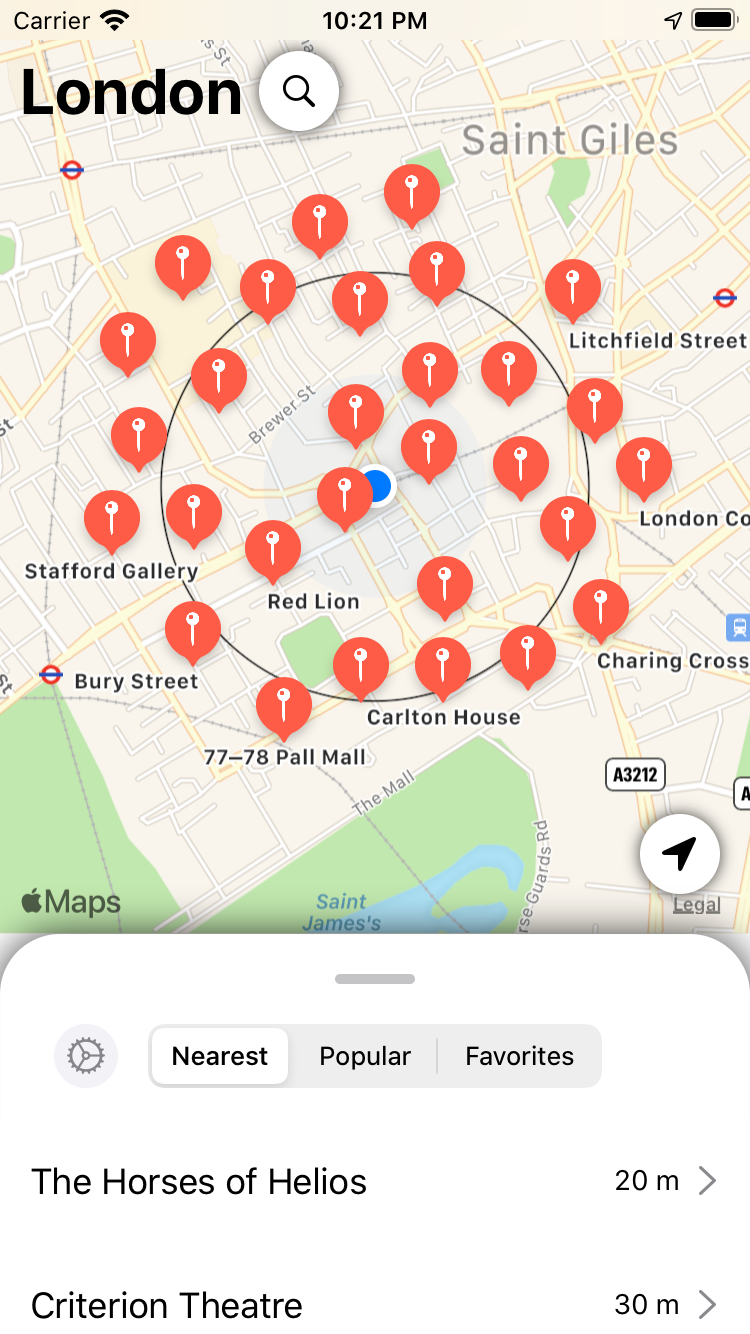
\includegraphics[width=0.98\linewidth]{/screenshot/light_nearest}
  	\label{fig:test1}
	\end{minipage}%
	\begin{minipage}{.5\textwidth}
  	\centering
  	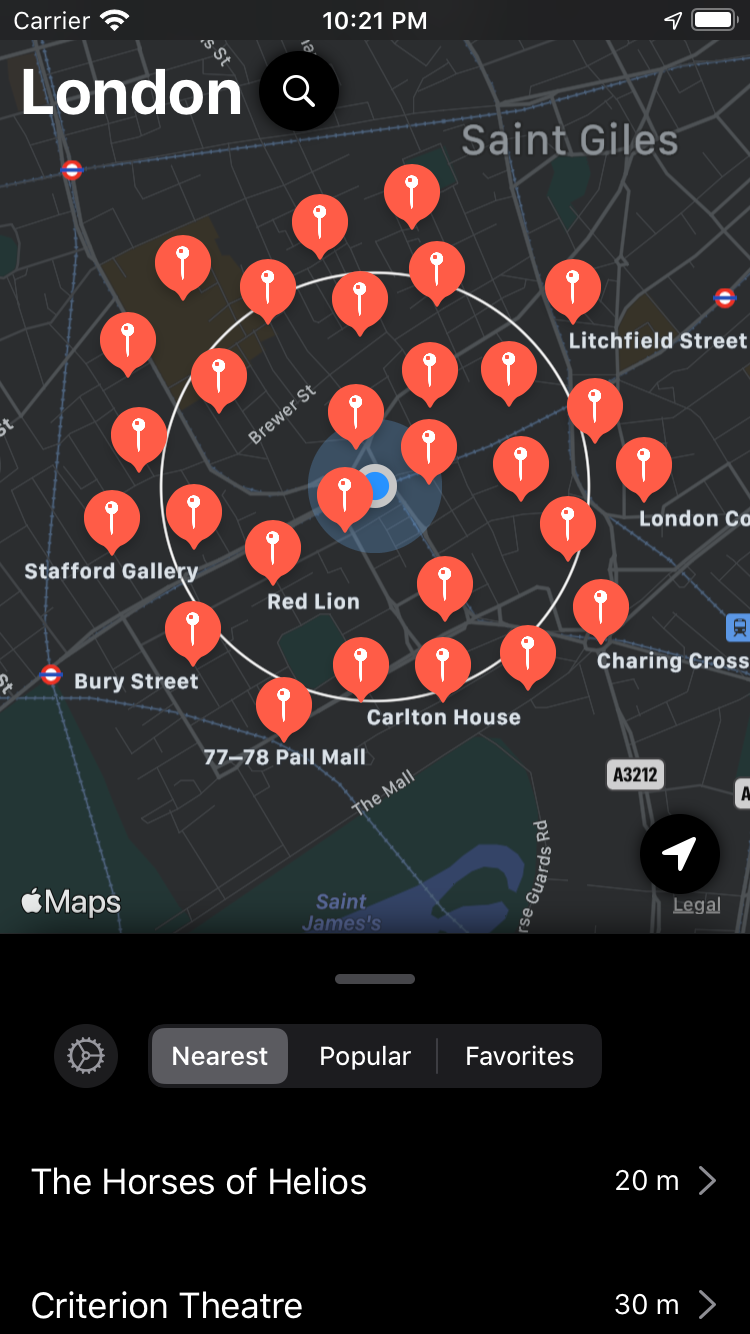
\includegraphics[width=0.98\linewidth]{/screenshot/dark_nearest}
  	\label{fig:test2}
	\end{minipage}
	\caption{Map view with nearest tab selected in both light and dark mode}
\end{figure}

This is the first view that appears when you open the app. Attractions, up to the maximum number selected, are displayed both in the maps and in the list below. In the list they are ordered by means of their distance to user current position.
\\In this view you can tap the city name to open the city detail view or an attraction to open the corresponding detail view. By pressing the search button, the user is presented with the common location search bar. Settings are reachable by pressing the gear button near the selectors.
\\The tab view for attraction list id resizable.

\subsection{Mapview - popular}
\begin{figure}[H]
	\centering
	\begin{minipage}{.5\textwidth}
  	\centering
  	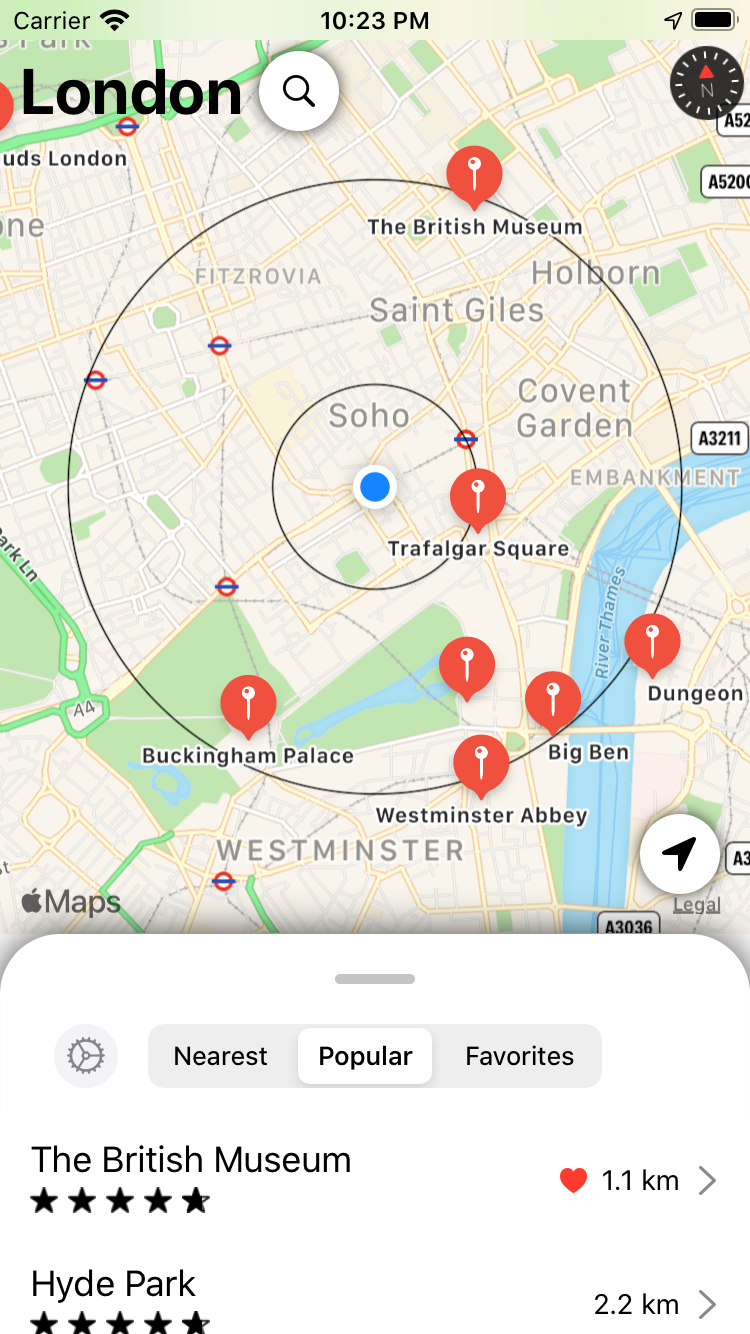
\includegraphics[width=0.98\linewidth]{/screenshot/light_popular}
  	\label{fig:test1}
	\end{minipage}%
	\begin{minipage}{.5\textwidth}
  	\centering
  	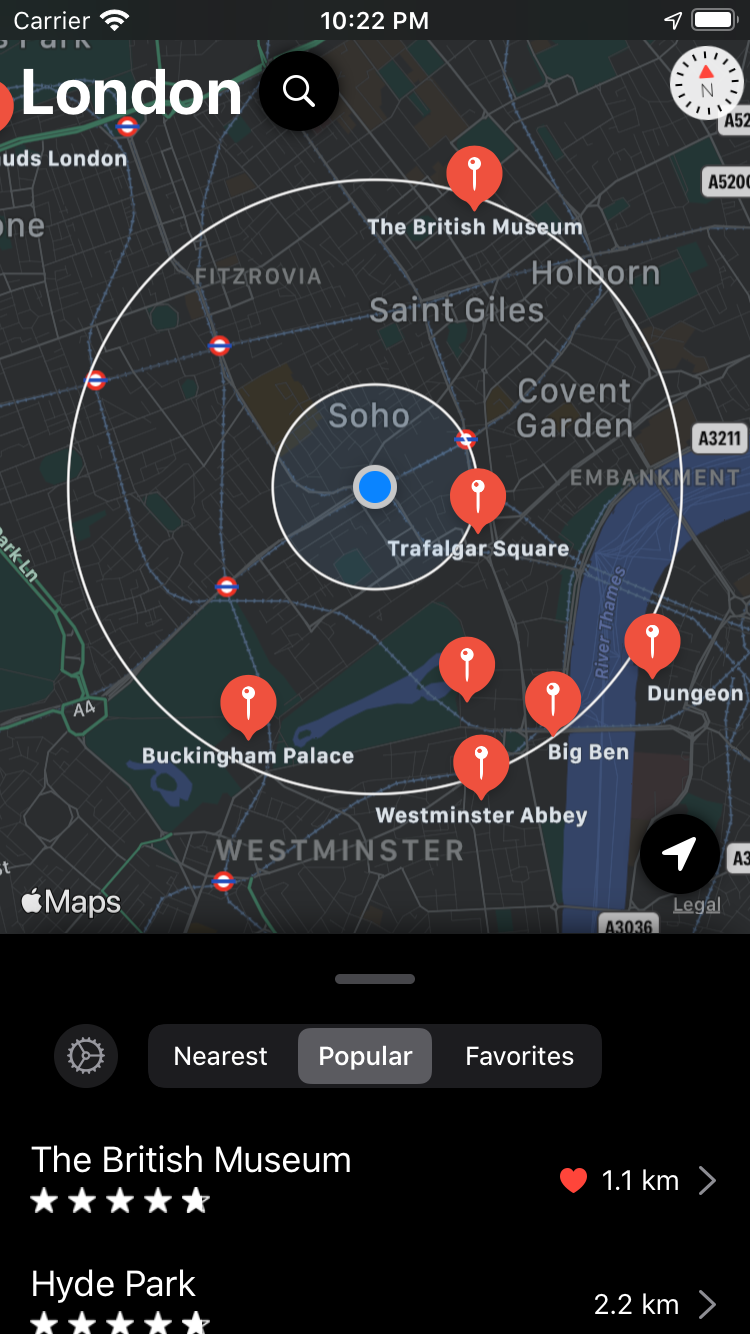
\includegraphics[width=0.98\linewidth]{/screenshot/dark_popular}
  	\label{fig:test2}
	\end{minipage}
	\caption{Map view with popular tab selected in both light and dark mode}
\end{figure}
Same as previous view, but here popular attraction tab is selected. Thus only most popular places are displayed. In the list, favourite items are identified by a hearth icon and the rating of each attraction is also displayed.
\\In this screenshot, circles that represent distance are more visible. They respectively represent the distance that the user can cover in 5 and 15 minutes of walking at her current walking speed.

\subsection{Mapview - favourite}
\begin{figure}[H]
	\centering
	\begin{minipage}{.5\textwidth}
  	\centering
  	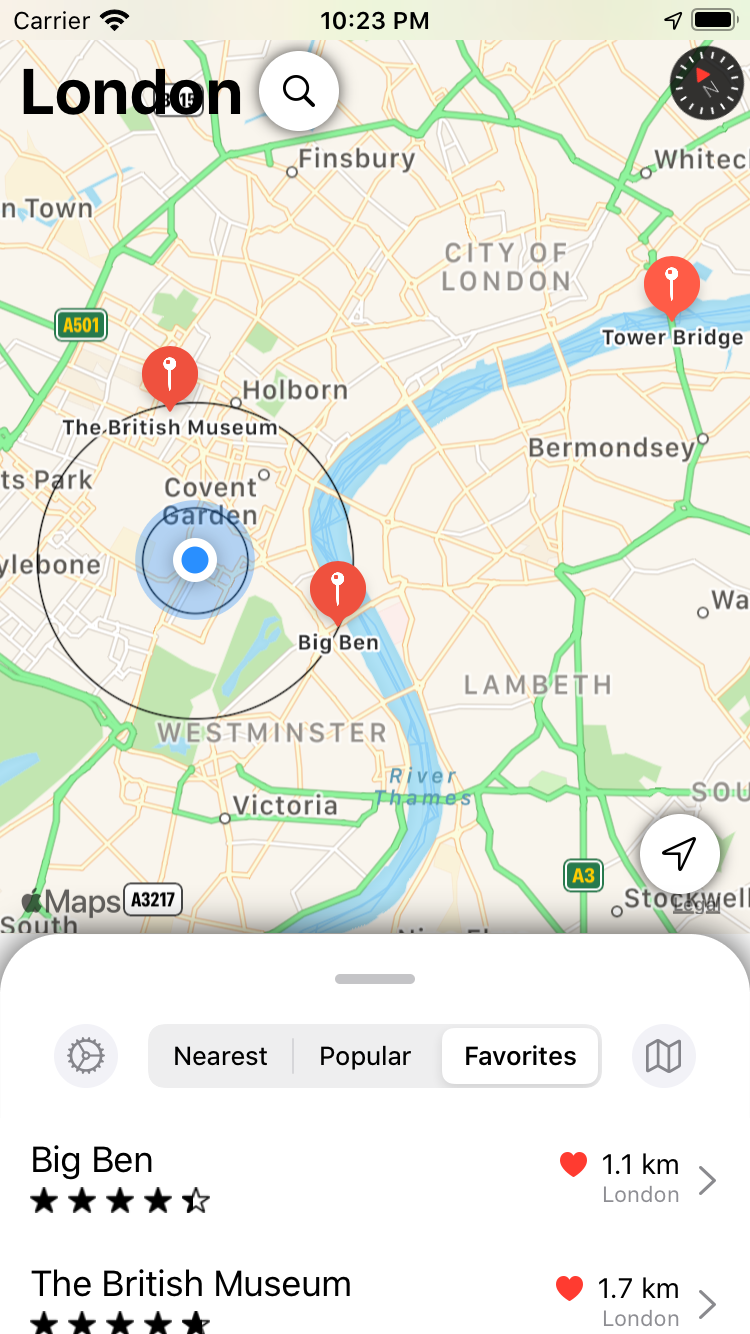
\includegraphics[width=0.98\linewidth]{/screenshot/light_favourite}
  	\label{fig:test1}
	\end{minipage}%
	\begin{minipage}{.5\textwidth}
  	\centering
  	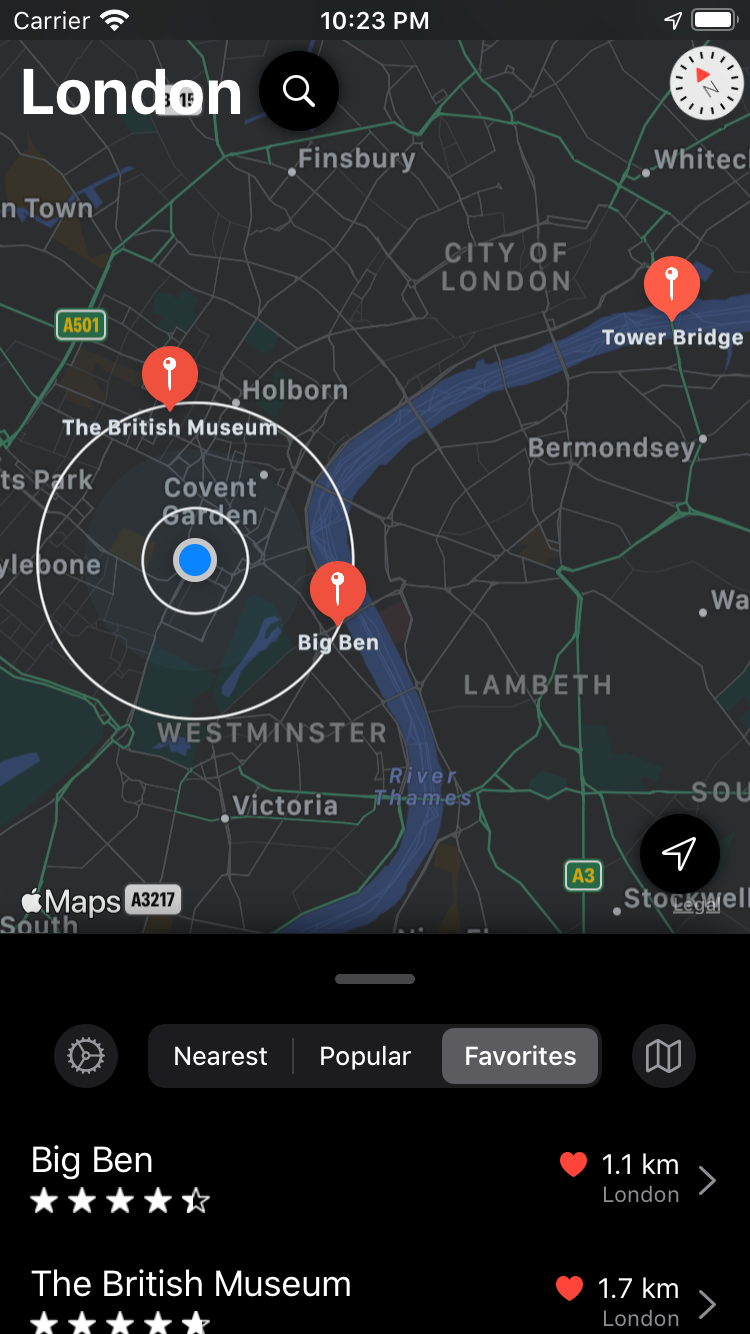
\includegraphics[width=0.98\linewidth]{/screenshot/dark_favourite}
  	\label{fig:test2}
	\end{minipage}
	\caption{Map view with favourite tab selected in both light and dark mode}
\end{figure}
Same as previous view, but here favourite attraction tab is selected. Since it's a global tab, they are grouped by city, that is also displayed. 
\\An additional button with a map is displayed, it lets the user to access the global view of favourite items.

\subsection{Global favourite view}
\begin{figure}[H]
	\centering
	\begin{minipage}{.5\textwidth}
  	\centering
  	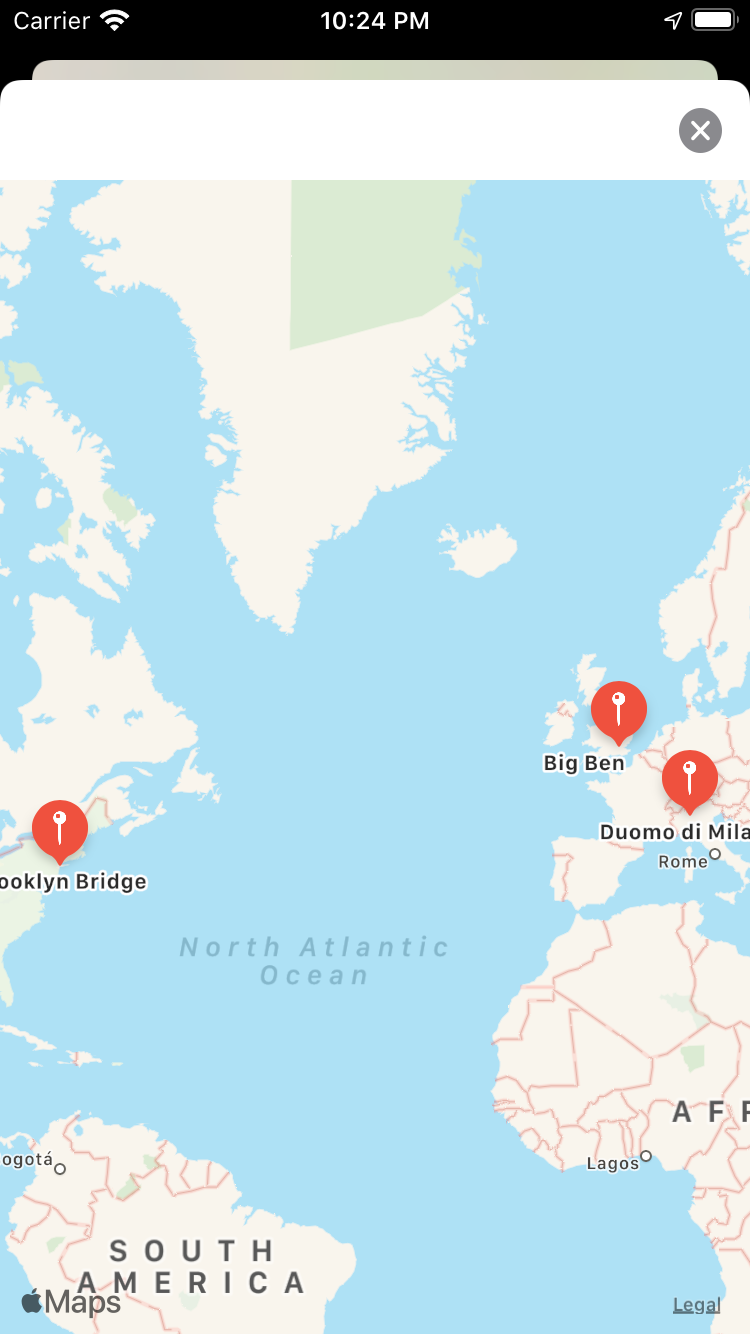
\includegraphics[width=0.98\linewidth]{/screenshot/light_worldwide}
  	\label{fig:test1}
	\end{minipage}%
	\begin{minipage}{.5\textwidth}
  	\centering
  	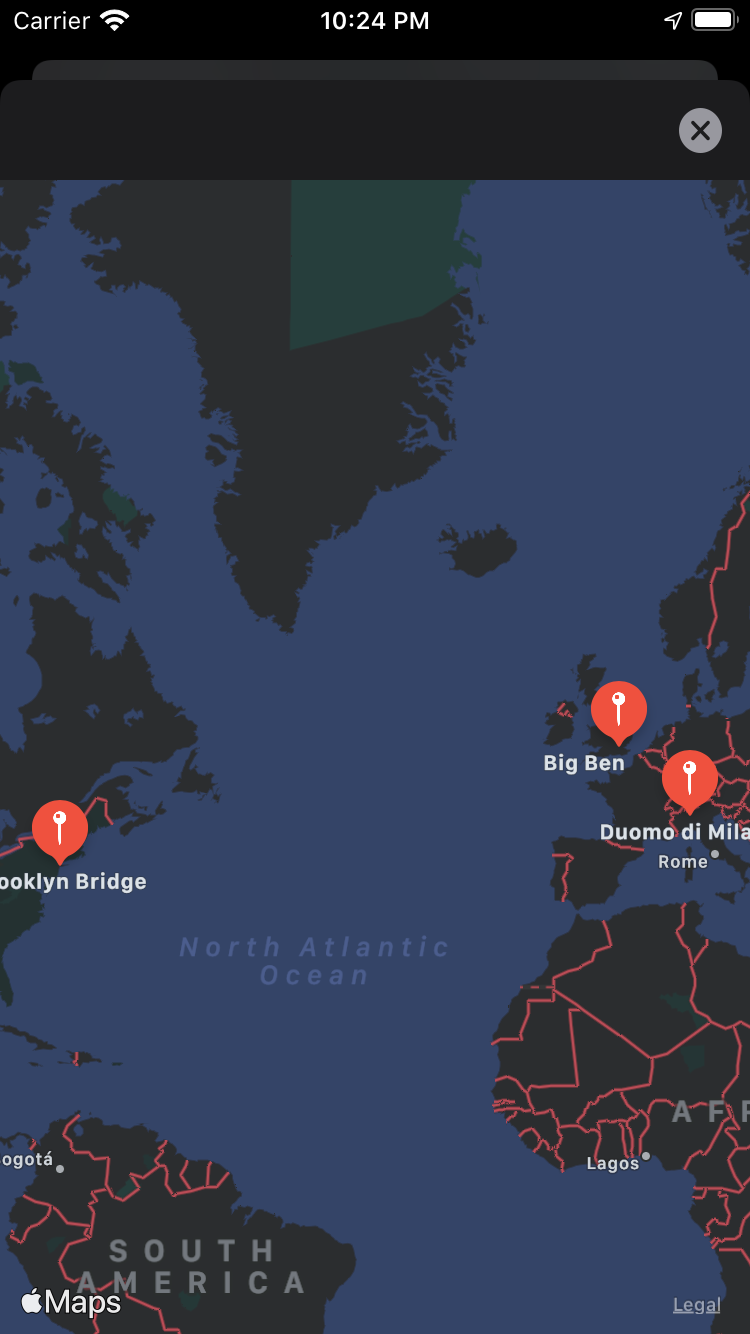
\includegraphics[width=0.98\linewidth]{/screenshot/dark_worldwide}
  	\label{fig:test2}
	\end{minipage}
	\caption{Favourite worldwide view in both light and dark mode}
\end{figure}
In this view, all user's favourite attractions are displayed in a map with fixed zoom. 

\subsection{Attraction detail view}
\begin{figure}[H]
	\centering
	\begin{minipage}{.5\textwidth}
  	\centering
  	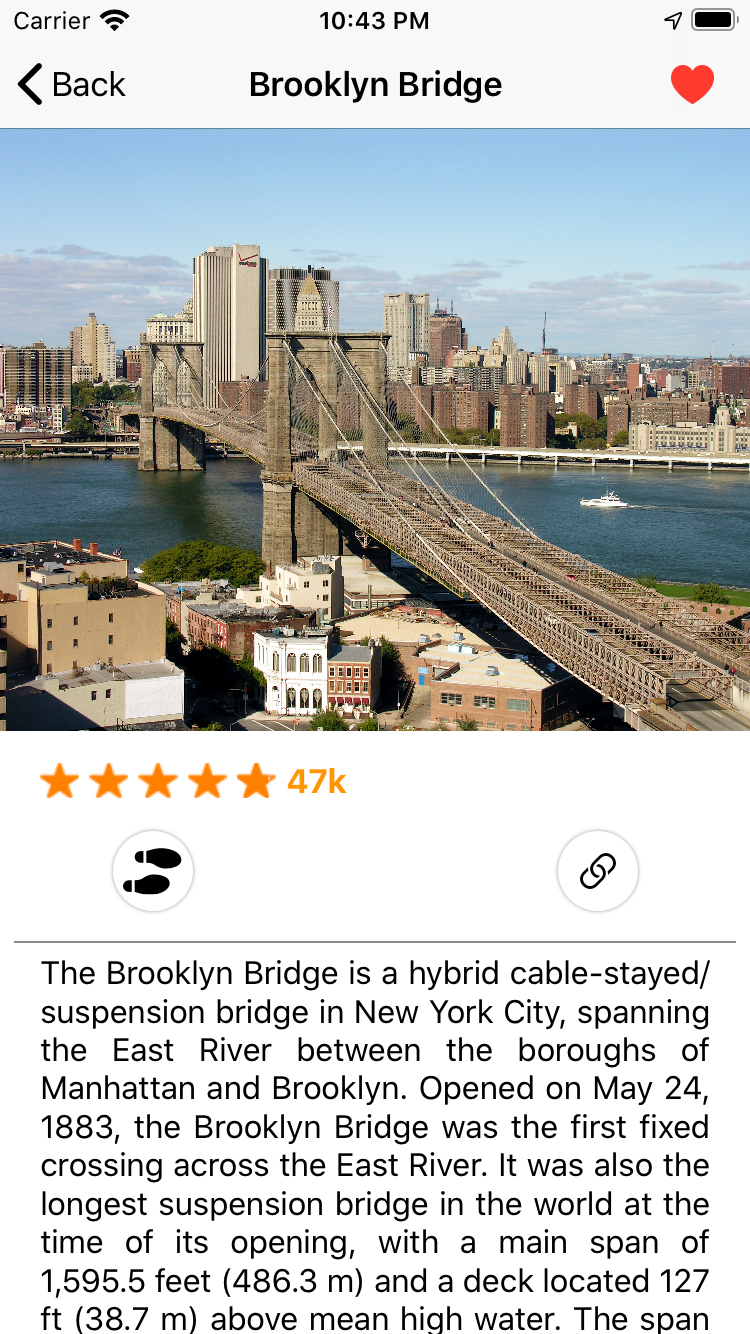
\includegraphics[width=0.98\linewidth]{/screenshot/light_detail_view}
  	\label{fig:test1}
	\end{minipage}%
	\begin{minipage}{.5\textwidth}
  	\centering
  	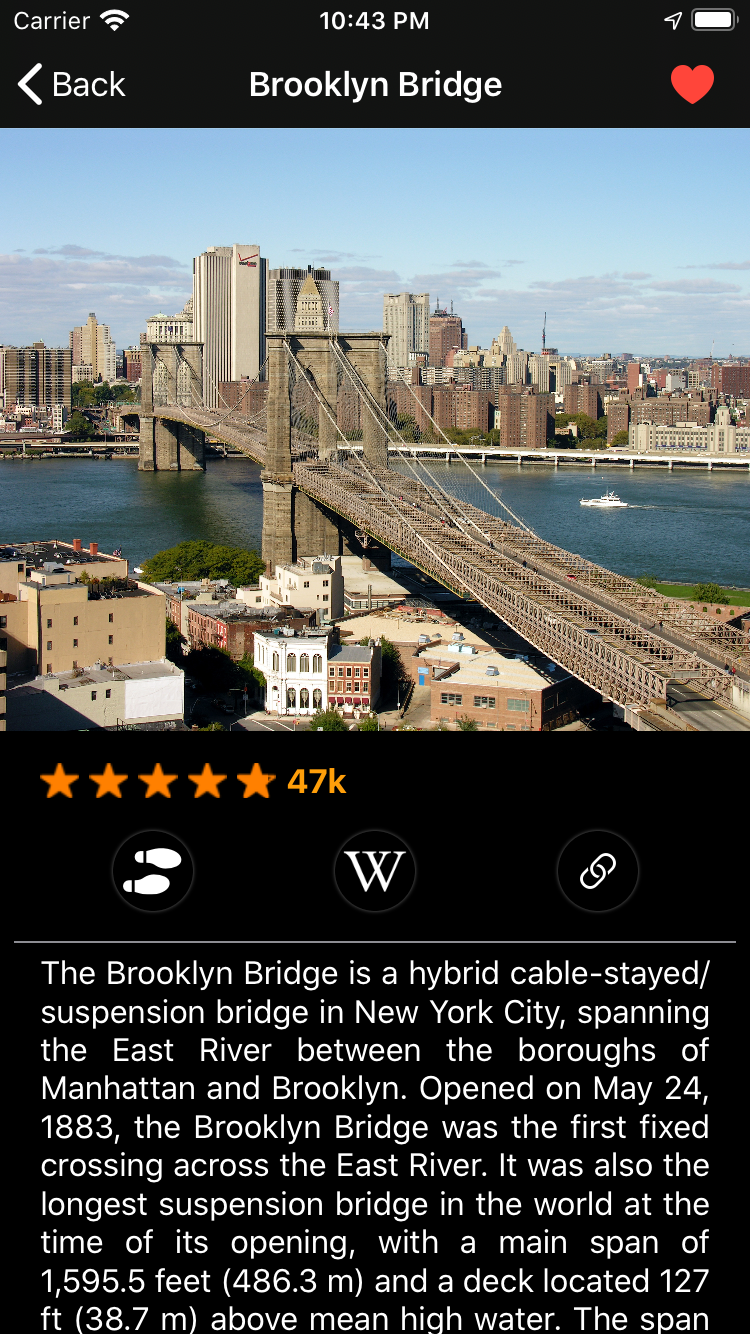
\includegraphics[width=0.98\linewidth]{/screenshot/dark_detail_view}
  	\label{fig:test2}
	\end{minipage}
	\caption{Attraction detail view in both light and dark mode}
\end{figure}

This is the detailed view that is presented when the user tap a specific attraction. A slideshow of picture of the attraction is displayed together with the rating (if available) and buttons that let you access the map direction, the complete Wikipedia Article and the related website.
In the navigation bar, the back button is available together with the hearth button that let the user favourite the attraction. The view is scrollable to display the entire place description extract. A detailed map with the specific attraction location is also provided at the end. 

\subsection{City detail view}
\begin{figure}[H]
	\centering
	\begin{minipage}{.5\textwidth}
  	\centering
  	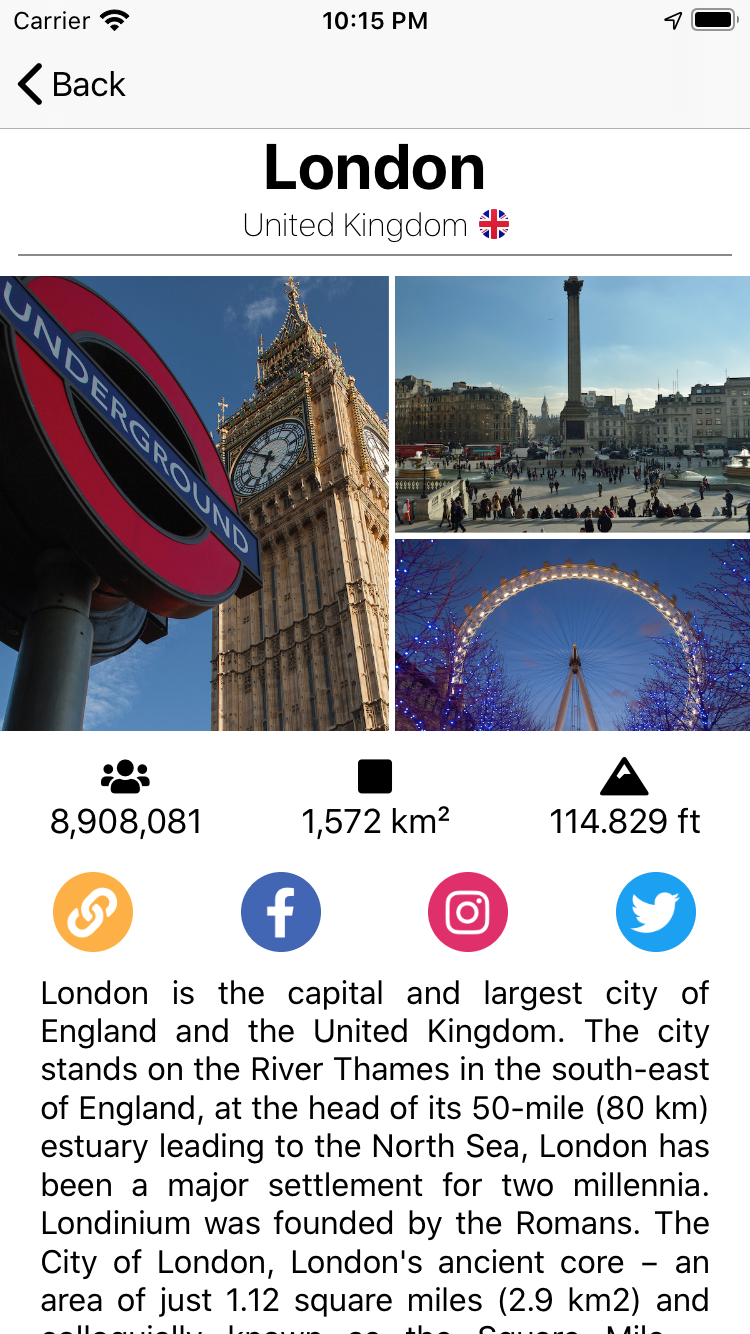
\includegraphics[width=0.98\linewidth]{/screenshot/light_city_detail_view}
  	\label{fig:test1}
	\end{minipage}%
	\begin{minipage}{.5\textwidth}
  	\centering
  	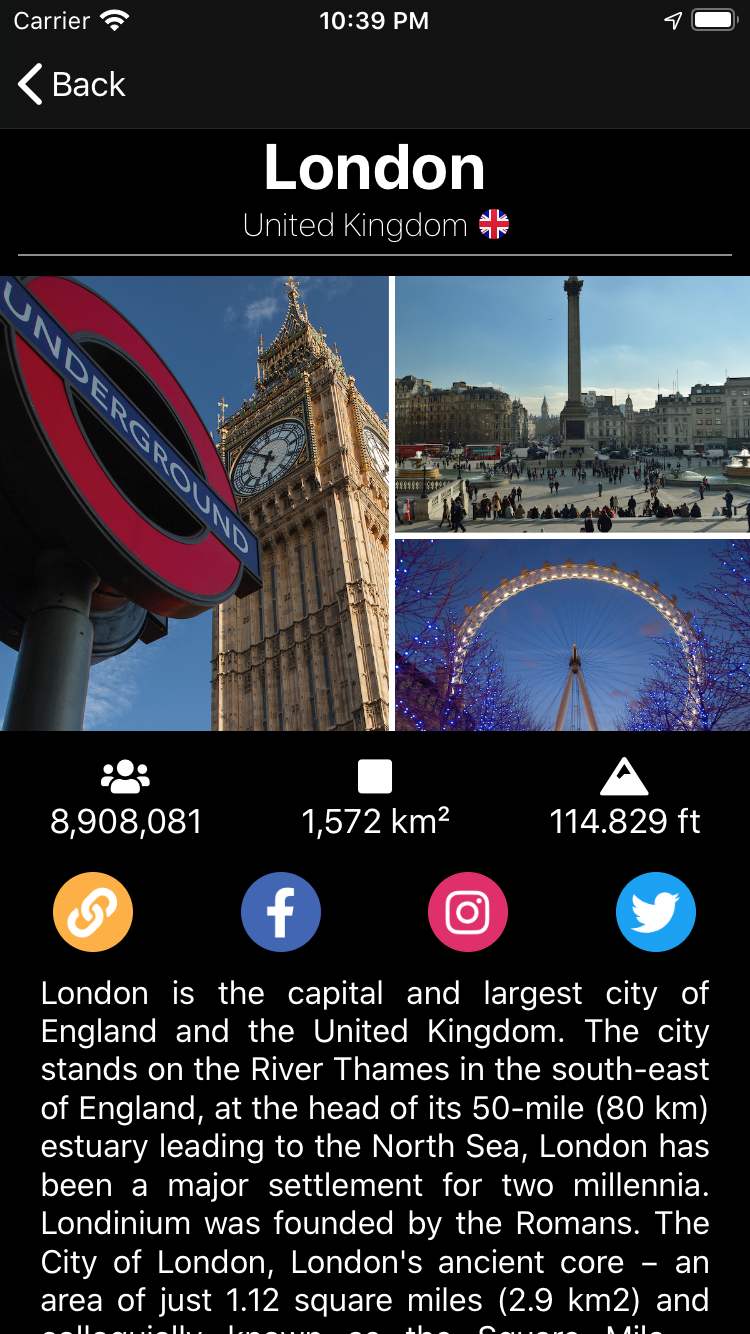
\includegraphics[width=0.98\linewidth]{/screenshot/dark_city_detail_view}
  	\label{fig:test2}
	\end{minipage}
	\caption{City detail view in both light and dark mode}
\end{figure}

This is the city detail view that is displayed when the user tap the city name in the main view. A pictures slideshow is displayed together with some information such as: population, area and altitude. A set of social link is retrieved and presented to the user. The view is scrollable and a summary description of the city is given.


\subsection{Settings view}
\begin{figure}[H]
	\centering
	\begin{minipage}{.5\textwidth}
  	\centering
  	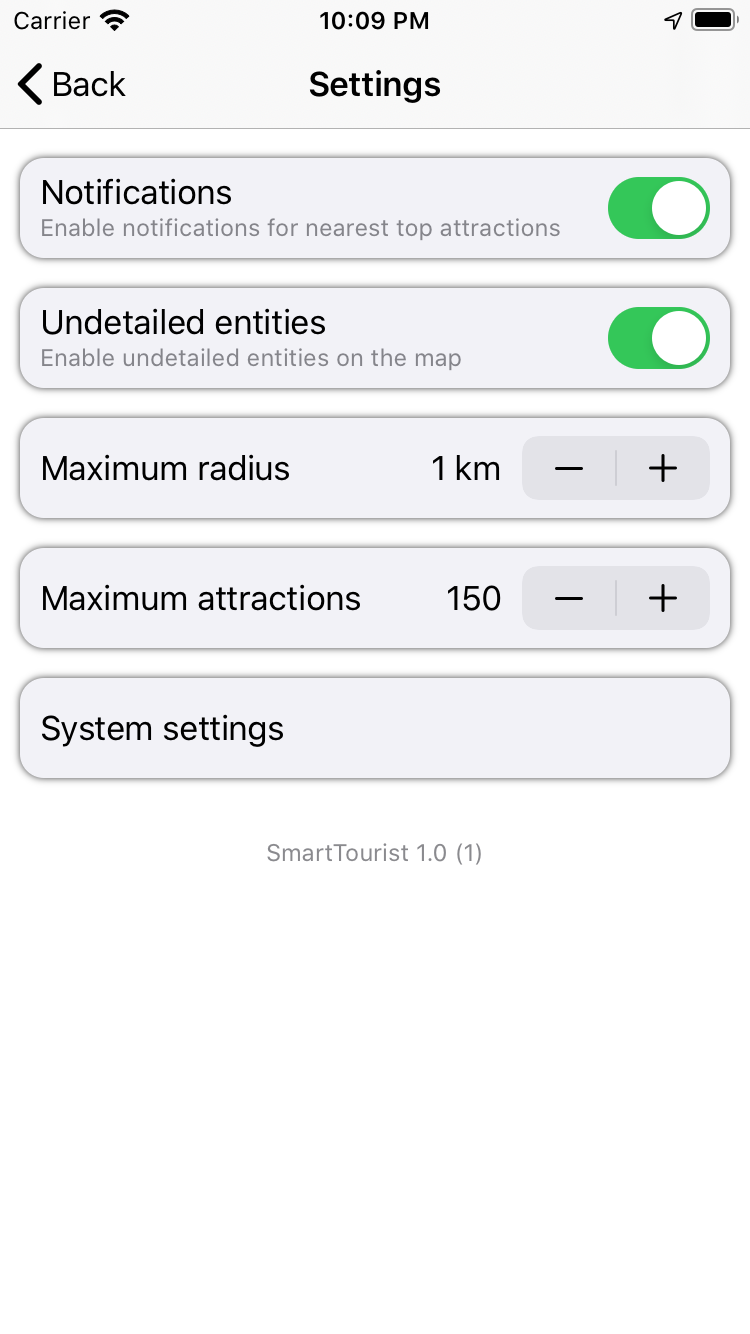
\includegraphics[width=0.98\linewidth]{/screenshot/light_settings}
  	\label{fig:test1}
	\end{minipage}%
	\begin{minipage}{.5\textwidth}
  	\centering
  	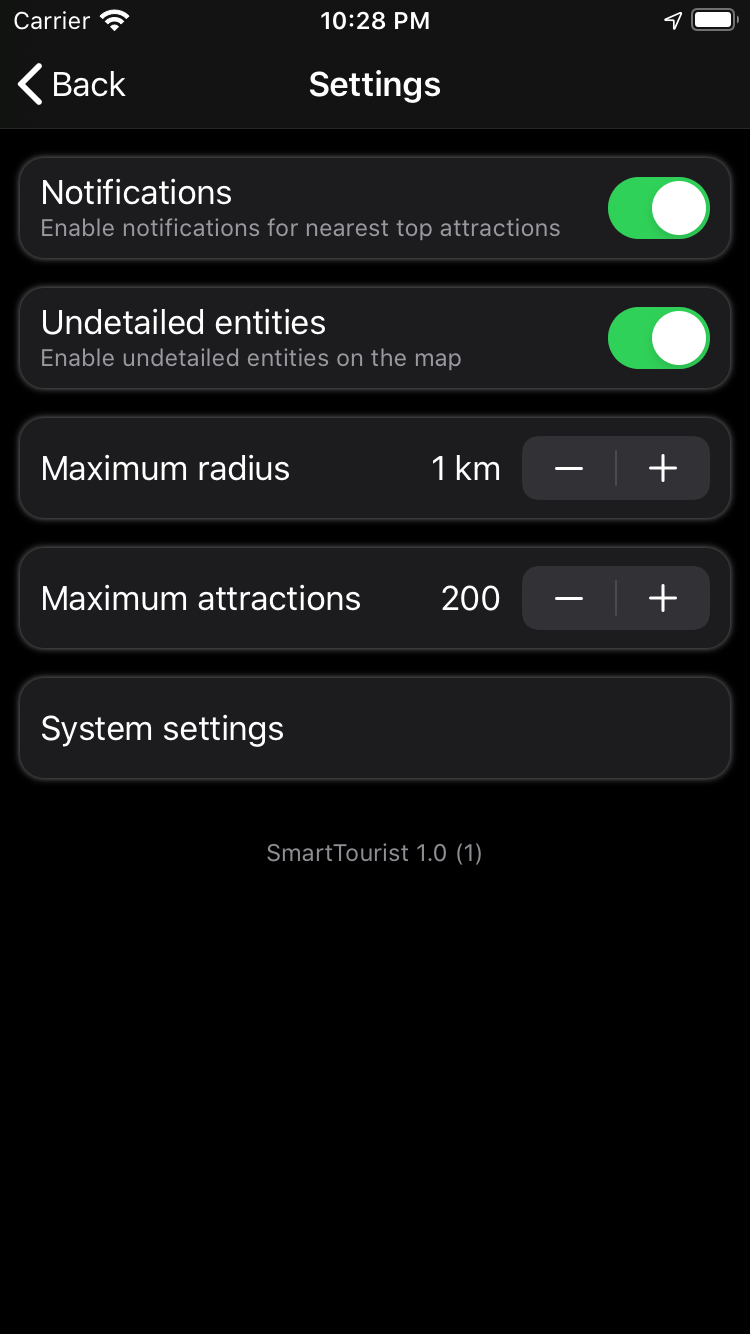
\includegraphics[width=0.98\linewidth]{/screenshot/dark_settings}
  	\label{fig:test2}
	\end{minipage}
	\caption{Settings view in both light and dark mode}
\end{figure}

Settings view is displayed when the gear icon on the main view is displayed. This is a quite standard settings view where some parameters about the application can be set.


\chapter{Notifications}




\chapter{Services and libraries}

\section{Internal libraries}

SmartTourist uses consistently internal libraries and services:

\begin{itemize}
	\item \textbf{\textit{MapKit}}: for location gathering and maps.
	\item \textbf{\textit{Core Motion}}: for accessing accelerometer, gyroscope, pedometer, and environment-related events.
\end{itemize}

\section{External services}

SmartTourist relies almost only on \textit{free data and services}. Here, it follows the description of the external services used.

\begin{itemize}
	\item \textit{\textbf{Wikipedia}}: all displayed attractions are taken from the Wikidata knowledge base. The given API is quite basic: attraction entries are retrieved with a SPARQL query embedded in a http API call. Details and pictures are retrieved with standard HTTP API calls from different endpoints.
		
		\begin{lstlisting}[language=sql, caption={SPARQL query for attraction retrieving}, captionpos=b]
		
		SELECT DISTINCT ?place ?placeLabel ?location ?image ?instance ?phoneNumber ?website ?wikipediaLink
        WHERE {
            SERVICE wikibase:label { bd:serviceParam wikibase:language "en, it" }
            SERVICE wikibase:around {
                ?place wdt:P625 ?location .
                bd:serviceParam wikibase:center "Point(\(location.longitude) \(location.latitude))"^^geo:wktLiteral .
                bd:serviceParam wikibase:radius "\(radius)" .
            }
            ?place wdt:P31 ?instance  .
        ?place wdt:P18 ?image .
        OPTIONAL {?place wdt:P1329 ?phoneNumber}.
        OPTIONAL {?place wdt:P856 ?website} .
        OPTIONAL {?wikipediaLink schema:about ?place;
            schema:inLanguage "en";
            schema:isPartOf [ wikibase:wikiGroup "wikipedia" ]} .
        }
		\end{lstlisting}
		
		\begin{lstlisting}[language=sql, caption={SPARQL query for city detail retrieving}, captionpos=b]
			SELECT DISTINCT ?city ?cityLabel ?country ?countryLabel ?population ?area ?elevation ?link ?facebookPageId ?facebookPlacesId ?instagramUsername ?twitterUsername ?image ?coatOfArmsImage ?cityFlagImage ?countryCode ?wikipediaLink WHERE {
            BIND( <http://www.wikidata.org/entity/\(cityId)> as ?city ).
            OPTIONAL {?city wdt:P17 ?country}.
            OPTIONAL {?city wdt:P1082 ?population}.
            OPTIONAL {?city wdt:P2046 ?area}.
            OPTIONAL {?city wdt:P2044 ?elevation}.
            OPTIONAL {?city wdt:P856 ?link}.
            OPTIONAL {?city wdt:P2013 ?facebookPageId}.
            OPTIONAL {?city wdt:P1997 ?facebookPlacesId}.
            OPTIONAL {?city wdt:P2003 ?instagramUsername}.
            OPTIONAL {?city wdt:P2002 ?twitterUsername}.
            OPTIONAL {?city wdt:P18 ?image}.
            OPTIONAL {?city wdt:P94  ?coatOfArmsImage}.
            OPTIONAL {?city wdt:P41 ?cityFlagImage}.
            OPTIONAL {?country wdt:P297 ?countryCode}.
            OPTIONAL {?wikipediaLink schema:about ?city;
              schema:inLanguage "en";
              schema:isPartOf [ wikibase:wikiGroup "wikipedia" ]}.
            SERVICE wikibase:label { bd:serviceParam wikibase:language "en". }
        }
		\end{lstlisting}
		
	\item \textit{\textbf{Google}}: Places ratings are the only data retrieved from Google services. This was due to the lack of a reliable free alternative. For the simplicity of the task, we decided not to rely on the Google SDK for iOS and to manually make request to the Google API.
\end{itemize}

\section{External libraries}

The app uses lots of third parties libraries the can be roughly divided into three kind: architectural libraries, back-end libraries and front-end libraries.

\begin{table}[h]
    \centering
    \def\arraystretch{1.3}
    \begin{tabular}{|c|c|m{9cm}|}
        \hline
        \textbf{Kind} & \textbf{Library} & \textbf{Description} \\ \hline
        \multirow{2}{*}{Architectural} & Katana & Katana is a modern Swift framework for writing iOS applications' business logic that are testable and easy to reason about. Katana is inspired by Redux. \\ \cline{2-3}
        & Tempura & Tempura is a holistic approach to iOS development, it borrows concepts from Redux (through Katana) and MVVM. \\ \hline
        \multirow{5}{*}{Back-end} & DeepDiff & DeepDiff tells the difference between 2 collections and the changes as edit steps. \\ \cline{2-3}
        & Fuse & Fuse is a super lightweight library which provides a simple way to do fuzzy searching. \\ \cline{2-3}
        & Alamofire & Alamofire is an HTTP networking library written in Swift. \\ \cline{2-3}
        & SigmaSwiftStatistics & It is a collection of functions that perform statistical calculations in Swift. It can be used in Swift apps for Apple devices and in open source Swift programs on other platforms. \\ \cline{2-3}
        & SwiftyXMLParser & Simple XML Parser implemented in Swift. \\ \hline
        \multirow{7}{*}{Front-end} & PinLayout & Extremely fast views layouting without auto layout. No magic, pure code, full control and blazing fast. Concise syntax, intuitive, readable and chainable. PinLayout can layouts UIView, NSView and CALayer. \\ \cline{2-3}
        & FlexLayout & Angular Flex Layout provides a sophisticated layout API using Flexbox CSS + mediaQuery. \\ \cline{2-3}
        & Cosmos & This is a UI control for iOS and tvOS written in Swift. \\ \cline{2-3}
        & ImageSlideshow & Customizable Swift image slideshow with circular scrolling, timer and full screen viewer. \\ \cline{2-3}
        & MarqueeLabel & MarqueeLabel is a UILabel subclass adds a scrolling marquee effect when the text of the label outgrows the available width. \\ \cline{2-3}
        & FontAwesome & Use Font Awesome in your Swift projects. \\ \cline{2-3}
        & FlagKit & Beautiful flag icons for usage in apps and on the web. \\ \hline
    \end{tabular}
\end{table}



\chapter{Testing}




\chapter{Effort spent}




\end{document}
